%
% zahlensysteme.tex
%
% (c) 2020 Prof Dr Andreas Müller, Hochschule Rapperswil
%
\section{Zahlensysteme
\label{buch:section:zahlensysteme}}
\rhead{Zahlensysteme}
Auf modernen Allzweck-Prozessoren steht eine ganze Reihe verschiedener
numerischer Datentypen mit unterschiedlichen Eigenschaften
bezüglich Geschwindigkeit und Fehlerverhalten zur Verfügung.
In diesem Abschnitt sollen sie vorgestellt und miteinander verglichen
werden.
Es gilt, den für eine Berechnung zweckmässigsten Typen zu wählen,
wobei Speicherbedarf, Laufzeit und Parallelisierbarkeit wesentliche
Aspekte sind.
\index{Speicherbedarf}%
\index{Laufzeit}%
\index{Parallelisierbarkeit}%

Microcontroller sind im Vergleich zu Allzweckprozessoren oft stark
\index{Microcontroller}%
eingeschränkt.
Meist sind nur Ganzahltypen mit oft sehr beschränkter Länge implementiert.
\index{Ganzzahltyp}%
Manchmal kann die Arithmetik-Einheit des Prozessors nicht einmal eine
Multiplikation in Hardware ausführen, sie muss in Software zeitaufwendig
nachgebildet werden.
\index{Arithmetik-Einheit}%
Für Floatingpoint-Operationen muss oft Bibliotheken zurückgegriffen
werden, die den Speicherbedarf erhöhen und langsam sind.
\index{Floatingpoint}%
\index{Bibliothek}%
Die Implementation von numerischen Berechnungen in eingebetteten Anwendungen
ist daher mit besonderen Herausforderungen konfrontiert.

Dieselbe Schwierigkeit haben auch Allzweck-Prozessoren, wenn die
Genauigkeitsanforderungen die Möglichkeiten der von der Prozessor-Hardware
implementierten Typen übersteigt.
Dieser Fall tritt beispielsweise bei Berechnungen in der Kryptographie auf,
wo oft mit Ganzzahlen mit Tausenden von Stellen gerechnet werden muss.
\index{Kryptographie}
Im Abschnitt~\ref{buch:subsection:mp} mit der GNU Multiprecision-Library
ein Beispiel einer solchen Bibliothek vorgestellt.
\index{GNU GMP}%
\index{Multiprecision-Library}%

%
% Zahlendarstellung bezüglich verschiedener Basen
%
\subsection{Zahlendarstellung bezüglich verschiedener Basen
\label{buch:subsection:basen}}
Allen Zahlensystemen gemeinsam ist die Positionsdarstellung.
\index{Positionsdarstellung}
Eine Zahl wird als Zeichenkette $x=x_nx_{n-1}\dots x_3x_2x_1x_0$
geschreiben,
wobei die Zeichen $x_i$ Ziffern mit $0 \le x_i < b$ sind.
$b$ ist die Basis des Zahlensystems.
\index{Basis}%
Der Wert der Zahl $x$ ist dann 
\[
x
=
\sum_{k=1}^n x_kb^k.
\]
Um die Basis deutlich zu machen, 
hängen wir die Basis als Index an eine Zahlendarstellung an.
Es ist also zum Beispiel
\[
1291_{10}
=
10100001011_2
=
1202211_3
=
2413_8
=
508_{16}.
\]
Bruchzahlen können analog dargestellt werden.
\index{Bruchzahl}%
Die Zeichenkette
\[
x = x_{n}x_{n-1}\dots x_2x_1x_0\texttt{.}x_{-1}x_{-2}x_{-3}\dots x_{-m}\dots
\]
hat den Wert
\[
x = \sum_{k=-m}^n x_kb^k.
\]
Die Zahl $\pi$ hat daher die Darstellungen
\index{$\pi$}%
\begin{align*}
\pi
&=
11.0010010000111111011011_2
\\
&=
10.01021101222201_3
\\
&=
3.11037552_8
\\
&=
3.1415926_{10}
\\
&=
3.243F6A_{16}
\end{align*}
in den Basen $2$, $3$, $8$, $10$ und $16$.
Eine grössere Basis erlaubt zwar eine kompaktere Darstellung, aber
für die Rechnung ermöglicht die binäre Darstellung die einfachste
und damit auch schnellste Implementation.

Man beachte, dass endliche Dezimalbrüche in anderen Basen durchaus
nicht mehr endlich zu sein brauchen.
So ist zum Beispiel
\begin{align*}
\frac12&= 0.5_{10} = 0.1_{2},
\\
\frac15&= 0.2_{10} = 0.001100110011\dots = 0.\overline{0011}_{2},
\\
\frac13&= 0.\overline{3}_{10} = 0.\overline{01}_{2}.
\end{align*}
Eine Konsequenz dieser Beobachtung ist, dass nur schon die Umwandlung
einer Dezimalzahl ins Binärsystem und die Rückumwandlung in eine Dezimalzahl
den Wert verändern kann.
Zum Beispiel\footnote{Dieses Beispiel wurde mit dem Programm
\texttt{format.cpp} aus dem Verzeichnis
\texttt{buch/chapters/experiments/limits} von \cite{buch:repo}
gerechnet.}
bewirkt der C++-Code
\begin{verbatim}
double	x = 0.2;
std::cout << x;
\end{verbatim}
dass der Compiler zunächst die Dezimalzahl $0.2$ in eine Binärzahl
verwandelt, diese Form wird im ausführbaren Code gespeichert.
\index{Compiler}%
Zur Laufzeit des Programms muss die I/O-Bibliothek dann die gespeicherte
Zahl wieder in eine Dezimalzahl verwandeln.
\index{Laufzeit}%
\index{Dezimalzahl}%
\index{Bibliothek}%
Für $x=0.5$ wäre das unproblematisch, da diese Zahl sowohl dezimal wie
auch binär ein endlicher Dezimalbruch ist.
Für $x=0.2$ tritt jedoch eine Abweichung auf, weil die im Code gespeichert
Binärzahl nicht exakt in $0.2$ zurückgewandelt werden kann.
\index{Binärzahl}%
Stattdessen erhält man abhängig vom Datentyp die abweichenden
Werte von Tabelle~\ref{buch:zahlensysteme:rundung}.
\begin{table}
\centering
\begin{tabular}{|>{\tt}r|>{$}r<{$}|>{$}r<{$}|}
\hline
\textrm{Typ}& 0.5\phantom{0000000000000000000}
                                    & 0.2\phantom{0000000000000000000}\\
\hline
float       & 0.50000000000000000000& 0.20000000298023223877\\
double      & 0.50000000000000000000& 0.20000000000000001110\\
long double & 0.50000000000000000000& 0.20000000000000001110\\
\hline
\end{tabular}
\index{\texttt{float}}%
\index{\texttt{double}}%
\index{\texttt{long double}}%
\caption{Nicht alle exakt darstellbaren Dezimalzahlen sind auch im
Binärsystem exakt darstellbar.
Die Zahl $0.2_{10}$ führt auf einee periodischee Binärzahl, die
beim Abspeichern gerundet werden muss.
Je nach Datentyp weicht der gerundete Wert mehr oder weniger stark ab.
\label{buch:zahlensysteme:rundung}}
\end{table}
Dass kein Unterschied zwischen \texttt{double} und \texttt{long double}
besteht, ist nur scheinbar. 
Multipliziert man $x$ mit $5$ vor dem Output, wird plötzlich ein
Unterschied sichtbar.

%
% Festkommazahlen
%
\subsection{Festkommazahlen
\label{buch:subsection:integers}}
Die bekanntesten Festkommazahlen sind die Ganzzahltypen, die jeder
Prozessor zum Beispiel für Adressierung, Zähler und Indizierung
benötigt.
\index{Festkommazahl}%
\index{Adressierung}%
\index{Indizierung}%
\index{Zähler}%
Damit ist auch bereits klar, dass man immer damit rechnen kann, dass
mindestens die Addition und die Subtraktion von ganzen Zahlen mit
Wortlängen implementiert sind, die der Prozessor zum Beispiel für
relative Adressierung braucht.
\index{Addition}%
\index{Subtraktion}%
\index{Wortlänge}%
\index{Prozessor}%
\index{Adressierung!relative}
Ebenso kann man davon ausgehen, dass jeder Kern eines Prozessors
eine Einheit für ganzzahlige Operationen hat, denn er könnte sonst
nicht einmal die minimal notwendigen Adressberechnungen durchführen.

\subsubsection{Addition}
Das Verfahren der ``schriftlichen Addition'', welches man in der Primarschule
lernt, funktioniert auch für die Berechnung einer Summe in jeder beliebigen
anderen Basis.
\index{schriftliche Addition}%
\index{Addition!schriftliche}%

\subsubsection{Vorzeichen}
\index{Vorzeichen}%
Ganzzahlen mit Vorzeichen können auf verschiedene Arten binär dargestellt
werden, weitgehend durchgesetzt hat sich für Festkommazahlen jedoch die
Zweierkomplement-Darstellung\footnote{Der Exponent einer Gleitkommanzahl
ist zwar auch eine Ganzzahl, er wird aber gemäss Standard IEEE 754
\index{IEEE 754}%
nach einem anderen Verfahren codiert, siehe dazu auch
Abschnitt~\ref{buch:subsection:floatinpoing}}.
\index{Zweierkomplement}%
In ihr werden 8-bit Zeichenketten wie folgt als Zahlen interpretiert:
\begin{align*}
\texttt{01111111}&= \phantom{-}127\\
\texttt{01111110}&= \phantom{-}126\\
\vdots\quad&\qquad\vdots\\
\texttt{00000010}&= \phantom{-00}2\\
\texttt{00000001}&= \phantom{-00}1\\
\texttt{00000000}&= \phantom{-00}0\\
\texttt{11111111}&= -\phantom{00}1\\
\texttt{11111110}&= -\phantom{00}2\\
\texttt{11111101}&= -\phantom{00}3\\
\vdots\quad&\qquad\vdots\\
\texttt{10000010}&=-126\\
\texttt{10000001}&=-127\\
\texttt{10000000}&=-128
\end{align*}
Diese Codierung ist in Hardware besonders leicht implementiertbar.
Ein Zähler für eine vorzeichenlose Ganzzahl von 8 bit Länge, initialisiert
mit \texttt{10000000} wird beim Hochzählen genau die Zahlen von $-128$
bis $127$ aufzählen.

Die Entgegengesetzte einer Zahl kann nach der folgenden Regel gefunden werden:
\index{entgegengesetzte Zahl}
\begin{enumerate}
\item Man nehme das Komplement jedes einzelnen Bits einer Zahl
\item Addiere 1.
\end{enumerate}
\begin{beispiel}
Die Zahl $-1291$ soll als 16-bit Ganzzahl in Zweierkomplement-Darstellung
geschrieben werden.
Zunächst wird die Binärdarstellung benötigt:
$1291_{10}= \texttt{0000010100001011}_2$.
\begin{enumerate}
\item Bits komplementieren: \texttt{1111101011110100}
\item $1$ addieren: \texttt{1111101011110101}
\qedhere
\end{enumerate}
\end{beispiel}

Die Addition vorzeichenbehafteter Ganzzahlen funktioniert für die
Zweierkomplementdarstellung nach dem bekannten Algorithmus für die
Addition.
Die Differenz $111-88$ kann man als Summe $111+(-88)$ schreiben.
Als 8-bit Binärzahlen sind die beiden Operanden
\texttt{01101111} und \texttt{10101000}.
Ihre Summe ist
\begin{center}
\begin{tabular}{>{\tt}r}
01101111\\
10101000\\
\hline
{\color{gray}}\,
00010111\\
\end{tabular}
\end{center}
Dabei ist zwar ein Überlauf aufgetreten, aber dieser kann ignoriert
werden.
Tatsächlich ist $23_{10}=10111_2$.
Der grosse Vorteil dieser Vorzeichenkonvention ist also, dass
für die Addition vorzeichenbehafteter Ganzzahlen in
Zweierkomplement-Darstellung die gleiche vorhandene Hardware verwendet
werden kann wie für die Addition vorzeichenloser Ganzzahlen.

\subsubsection{Multiplikation und Division}
Man kann allerdings nicht davon ausgehen, dass ein Prozessor auch
die Multiplikation von ganzen Zahlen und erst recht die Division
von ganzen Zahlen implementiert.
\index{Multiplikation}%
\index{Division}%
In den meisten Fällen benötigt der Prozessor nur die Multiplikation
mit kleinen Zweierpotenzen, die sich viel effizienter als
Verschiebeoperationen durchführen lassen.
\index{Zweierpotenz}%
\index{Verschiebeoperation}%

\subsubsection{Nachkommateil}
\index{Nachkommateil}%
Bisher wurden ausschliesslich Ganzzahlen betrachtet.
Man kann diese Ganzzahlen aber auch als rationale Zahlen mit einem
Nachkommateil fester Länge betrachten.
\index{rationale Zahl}%
\index{Zahl!rationale}%
Man könnte sich zum Beispiel nach den ersten 8 bit einer 16-bit Zahl
ein Komma denken und die nachfolgenden Bits als Bruchteil
betrachten.
Die Bitfolge \texttt{0000000110010000} muss dann als
\[
00000011.00100000_2
=
3.125_{10}
\]
interpretiert werden.
An den Algorithmen für Addition und Subtraktion ändert sich nichts,
es ist daher keine neue Hardware für die Implementation dieser
Operationen notwendig, die Ganzzahloperationen reichen aus.
\index{Algorithmus}%

Etwas komplizierter ist die Sache bei der Multiplikation.
Nehmen wir an, dass wir mit 8-bit Festkomma-Zahlen arbeiten mit
einem Nachkommateil von 4 bits. 
Wir möchten das Produkt $3.125\cdot 2.0625$ berechnen.
Die Binärdarstellungen dieser Zahlen sind
$3.125_{10}=11.001_{2}$ und $2.0625_{10}= 10.0001_{2}$.
Das Produkt der 8-bit Ganzzahlen \texttt{00110010} und \texttt{00100001}
wird mehr Platz beanspruchen, im schlimmsten Fall 16 bit:
\[
\texttt{00110010}_2\cdot\texttt{00100001}_2
=
\texttt{0000011001110010}_2.
\]
In den Faktoren sind die letzten 4 Stellen jeweils als Nachkommateil
zu unterpretieren, also sind im Produkt die letzten 8 Stellen als
Nachkommateil zu interpretieren.
Das Produkt, wieder als 8-bit Festkommazahl geschrieben ist daher
\[
\texttt{0011.0010}_2\cdot\texttt{0010.0001}_2
=
\texttt{00000110.01110010}_2
\approx
\texttt{0110.0111}_2
\]
Auch für die Multiplikation ist keine neue Hardware erforderlich,
doch muss das Resultat entsprechend mit Schiebeoperationen wieder
so formattiert werden, dass das Komma an der ``richtigen'' Stelle
landet.
\index{Schiebeoperation}%

Mit den Ganzzahl-Operationen einer CPU lassen sich also auch sehr
schnelle Festkomma-Ope\-ra\-tio\-nen realisieren.

\subsubsection{Vor- und Nachteile von Festkommazahlen}
\begin{itemize}
\item[$\oplus$]
Eine beliebige relle Zahl muss bei der Darstellung als Festkommazahl
um Maximal die Hälfte der Wertigkeit der letzten Stelle gerundet werden.
Dieser absolute Fehler ist konstant.
\index{absoluter Fehler}%
\index{Fehler!relativer}%
\item[$\oplus$]
Operationen sind typischerweise deutlich schneller als
mit Gleitkommazahlen vergleichbarer Grösse.
Dies gilt insbesondere dann, wenn die Operationen zum Teil in Software 
realisiert werden müssen.
\item[$\oplus$] Die Addition und Subtraktion sind von derart elementarer
Bedeutung für einen CPU-Kern, dass jeder Kern mindestens eine Einheit
für Ganzzahl-Operationen hat.
In einer Multicore-CPU kann man daher davon ausgehen, dass Festkomma-Operationen
sich auf verschiedenen Cores nicht gegenseitig behindern.
\index{Multicore-CPU}%
\item[$\ominus$] Kleine Zahlen können nur mit wenigen signifikanten
Stellen dargestellt werden.
\index{signifikant}%
\item[$\ominus$] Schon für mässig grosse Zahlen ist Überlauf möglich.
\index{Überlauf}%
\end{itemize}

%
% Gleitkommazahlen
%
\subsection{Gleitkommazahlen
\label{buch:subsection:floatinpoing}}
Gleitkommazahlen erweitern den Bereich der darstellbaren Zahlen dadurch,
dass sie zu einer Festkommazahl einen Exponentialfaktor hinzunehmen.
\index{Exponentialfaktor}%
\index{Gleitkommazahl}%
Eine Gleitkommazahl $x$ ist also von der Form
\[
x = m \cdot b^k.
\]
$m$ heisst Mantisse, $b$ ist die Basis und $k$ ist der
Exponent, üblicherweise eine kleine Ganzzahl.
\index{Mantisse}%
\index{Exponent}%
\index{Basis}%
Die Mantisse wird typischerweise so strukturiert, dass genau eine 
Stelle vor dem Komma steht.
Im Dezimalsystem sind also
\[
1291
=
1.291\cdot 10^{3},
\quad
\gamma = 5.772156649\cdot 10^{-1},
\quad
N_A
=
6.0221476\cdot 10^{23}
\]
korrekte Gleitkommazahlen.

Die meisten heutigen Prozessoren rechnen ausschliesslich binär.
\index{binär}%
Sowohl für die Mantisse wie für den Exponenten wird daher eine
Binärdarstellung verwendet, die Basis ist $b=2$.
Da die einzige Stelle vor dem Komma eine \texttt{1} sein muss, wird
sie normalerweise nicht gespeichert.
Das Vorzeichen der Zahl wird separat gespeichert.
\index{Vorzeichen}%

Der 32 bit umfassende Gleitkommatyp \texttt{float} hat eine Mantisse
von 24 bit, wovon aber nur 23 Bit gespeichert werden müssen.
\index{\texttt{float}}%
Von den verbleibenden 9 bit wird eines als Vorzeichen verwendet und
8 als Exponent.
Mit einer 8 bit Ganzzahl lassen sich die Zahlen von 0 bis 255 darstellen.
Um negative Exponenten zu ermöglichen, muss 127 subtrahiert werden.
Die 8 Exponenten-bits codieren also die Exponenten $-127$ bis $128$.

Die Zahl
\[
\pi 
=
3.14159265_{10}
=
\texttt{11.0010100110001011000010}_2
=
\texttt{1.10010100110001011000010}_2\cdot 2^{1}
\]
kann daher als \texttt{float}-Gleitkommazahl wie folgt gespeichert werden:
\begin{center}
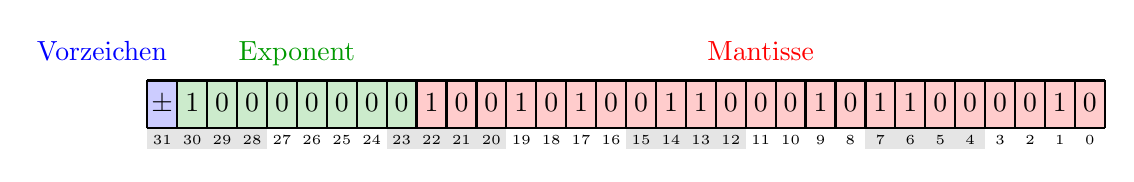
\begin{tikzpicture}[>=latex,thick,scale=0.38]

\definecolor{darkgreen}{rgb}{0,0.6,0}
\fill[color=blue!20]      (0,-0.8) rectangle (1,0.8);
\fill[color=darkgreen!20] (1,-0.8) rectangle (9,0.8);
\fill[color=red!20]       (9,-0.8) rectangle (32,0.8);

\node[color=blue]      at ( 1  ,0.8) [above left] {Vorzeichen\strut};
\node[color=darkgreen] at ( 5  ,0.8) [above] {Exponent\strut};
\node[color=red]       at (20.5,0.8) [above] {Mantisse\strut};

\fill[color=gray!20] ( 0,-0.8) rectangle ( 4,-1.5);
\fill[color=gray!20] ( 8,-0.8) rectangle (12,-1.5);
\fill[color=gray!20] (16,-0.8) rectangle (20,-1.5);
\fill[color=gray!20] (24,-0.8) rectangle (28,-1.5);

\foreach \k in {0,...,31}{
	\node at ({31.5-\k},{-1.2}) {\tiny \k};
}

\draw (0,0.8)--(32,0.8);
\foreach \x in {0,...,32}{
	\draw (\x,-0.8)--(\x,+0.8);
}
\draw (0,-0.8)--(32,-0.8);

\def\feld#1#2{
\node at ({#1+0.5},0) {$\mathstrut #2$};
}

\feld{0}{\pm}

\feld{1}{1}
\feld{2}{0}
\feld{3}{0}
\feld{4}{0}
\feld{5}{0}
\feld{6}{0}
\feld{7}{0}
\feld{8}{0}

\feld{9}{1}
\feld{10}{0}
\feld{11}{0}
\feld{12}{1}
\feld{13}{0}
\feld{14}{1}
\feld{15}{0}
\feld{16}{0}
\feld{17}{1}
\feld{18}{1}
\feld{19}{0}
\feld{20}{0}
\feld{21}{0}
\feld{22}{1}
\feld{23}{0}
\feld{24}{1}
\feld{25}{1}
\feld{26}{0}
\feld{27}{0}
\feld{28}{0}
\feld{29}{0}
\feld{30}{1}
\feld{31}{0}

\end{tikzpicture}
\end{center}
Die Ganzzahl $\texttt{10000000}_2=128_{10}$ im Exponentenfeld
muss um $127$ verringert werden um den Exponenten $1$ zu ergeben.

Die grösste und kleinste mit einem \texttt{float} darstellbare positive
Zahl ist somit
\begin{align*}
\texttt{1.11111111111111111111111}_2 \cdot 2^{\phantom{-}128}
&=
3.4028232_{10}\cdot 10^{\phantom{-}38}
\\
\texttt{1.00000000000000000000000}_2 \cdot 2^{-127}
&=
5.8774717_{10}\cdot 10^{-39}
\end{align*}
Den 24 binären Mantissenbits entsprechen gut 7 Dezimalstellen.

Genau genommen können noch etwas kleinere Zahlen dargestellt werden, wenn
man auf die Konvention verzichtet, dass vor dem Komma eine \texttt{1}
stehen muss.
Man nennt solche noch kleineren Zahlen {\em denomormalisiert}.
\index{denormalisiert}%
Da das Floatingpoint-Format immer auch eine implizite führende \texttt{1}
beinhaltet, braucht es zusätzliche Konventionen für denomarmalisierte Zahlen,
die die Abwesenheit der \texttt{1} signalisieren (Siehe auch den
Abschnitt Denormalisierung auf
Seite~\pageref{buch:zahlensysteme:denormalisierung}).
\index{Konvention!für denormalisierte Zahlen}%
\index{Denormalisierung}%

\begin{table}
\centering
\renewcommand\arraystretch{1.15}
\begin{tabular}{|l|>{$}l<{$}|>{$}l<{$}|>{$}l<{$}|}
\hline
&\texttt{float}&\texttt{double}&\texttt{long double}\\
\hline
kleinste darstellbare Zahl    &
	1.17549\cdot 10^{-38}&2.22507\cdot 10^{-308}&3.3621\cdot 10^{-4932}\\
grösste darstellbare Zahl     &
	3.40282\cdot10^{38} &1.79769\cdot10^{308} &1.18973\cdot10^{4932}\\
$\varepsilon$                 &
	1.19209\cdot 10^{-7}&2.22045\cdot 10^{-16}&1.0842\cdot 10^{-19}\\
kleinster Exponent            & -125&-1021&-16381\\
grösster Exponent             & 128&1024&16384\\
kleinste denormalisiert Zahl: &
	1.4013\cdot 10^{-45}&4.94066\cdot 10^{-324}&3.6452\cdot 10^{-4951}\\
\hline
\end{tabular}
\index{$\varepsilon$}
\caption{Eigenschaften der Gleitkommatypen \texttt{float}, \texttt{double}
und \texttt{long double}.
Die Zeile $\varepsilon$ ist die Differenz zwischen 1 und der kleinsten
darstellbaren Zahl, die grösser ist als $1$.
\index{kleinste darstellbare Zahl}%
Einzelne Exponentenwerte haben eine spezielle Bedeutung (siehe Text),
daher fallen die kleinstmöglichen Exponenten grösser aus als aufgrund
ihrer Bitlänge zu erwarten ist.
\label{buch:table:limits}}
\end{table}


\begin{table}
\centering
\begin{tabular}{|l|c|c|c|c|}
\hline
Typ&Bytes&Mantisse&Exponent&IEEE-754\\
\hline
\texttt{half},
\texttt{binary16}    &\phantom{0}2& \phantom{0}10 & \phantom{0}5     & * \\
\texttt{float},
\texttt{binary32}    &\phantom{0}4& \phantom{0}23 & \phantom{0}8     & * \\
\texttt{extended} 
                     &\phantom{0}5& \phantom{0}29 & 10               &   \\
\texttt{double},
\texttt{binary64}    &\phantom{0}8& \phantom{0}52 & 11               & * \\
\texttt{double extended},
\texttt{long double} &          10& \phantom{0}63 & 15               & * \\
\texttt{quad}
\texttt{binary128}   &          16& 112           & 15               & * \\
\texttt{binary256}   &          32& 236           & 19               & * \\
\hline
\end{tabular}
\caption{Übliche Gleitkommatypen mit Länge der Mantisse und des Exponenten.
Die meisten Compiler implementieren nur \texttt{float} und \texttt{double},
manchmal auch noch \texttt{long double}.
Die im Standard IEEE 754-2008 definierten Typen sind in der letzten Spalte
mit einen $*$ versehen.
\index{IEEE 754}%
\label{buch:table:ieee754}}
\end{table}

\subsubsection{Gebräuchliche Formate}
Der 1985 verabschiedete Standard IEEE~754 beschreibt die heute gebräuchlichen
Implementation von Gleitkommatypen abschliessend.
\index{IEEE~754}
Damit ist gewährleistet, dass numerische Rechnungen auf verschiedenen
Prozessoren reproduzierbare Resultate geben.

Die C++-Standardbibliothek bietet im \texttt{<limits>} Header die Möglichkeit, 
Informationen über die Datentypen zu erhalten.
\index{C++}%
\index{\texttt{<limits>}}%
In Tabelle~\ref{buch:table:limits} sind die Eigenschaften der
gebräuchlichsten Typen zusammengestellt.
Allerdings offenbart sich hier auch ein Problem dieser Implementation
von \texttt{<limits>}.
Wie wir weiter unten sehen werden, definiert der IEEE 754 Standard
Werte für $\pm\infty$, die kleiner sind als die angegebenen
maximalen Werte.

Aktuelle Compiler unterstützen typischerweise die Gleitkomma-Typen
\texttt{float}, \texttt{double} und \texttt{long double}.
\index{Compiler}%
\index{\texttt{float}}%
\index{\texttt{double}}%
\index{\texttt{long double}}%
Bei Microkontrollern, wo Berechnungen mit der hohen Präzision
eines \texttt{double} nur schon wegen des Platzedarfs der Werte
und des Zeitbedarfs für die Operationen kaum sinnvoll sind, ist oft
nur der \texttt{float}-Typ implementiert.
\index{Microcontroller}%
Der GNU-Compiler für die 8-bit AVR-Prozessorfamilie stellt behandelt
zum Beispiel \texttt{double} genau gleich wie \texttt{float}.
\index{GNU-Compiler}%
\index{AVR}%
Graphikkarten unterstützen oft noch einen halben Gleitkommatyp
\texttt{binary16}, dessen Genauigkeit für die Darstellung von 3D-Objekten
ausreichend ist.
\index{Graphikkarte}%
\index{\texttt{binary16}}%
\index{3D}%

\subsubsection{Rundung}
Der IEEE 754 Standard schreibt auch vor, wie Resultate gerundet werden
müssen.
\index{Rundungs-Regel}
Bei vielen Operationen entstehen Resultate, die einen längeren 
Nachkommateil haben als in das gegebene Gleitkommaformat passt,
das Resultat muss gerundet werden.
\index{Rundung}%
Der Standard kennt fünf verschiedene Rundungsverfahren und empfiehlt,
dass die Funktionen wie Wurzeln, Exponentialfunktionen,
trigonometrische Funktionen und viele weitere so implementiert werden 
müssen, dass das Resultat korrekt gerundet ist.
\index{Wurzel}%
\index{Exponentialfunktion}%
\index{trigenometrische Funktion}%
\index{Funktion!trigonometrische}%
Damit ist gemeint, dass das Resultat entsteht, in dem auf das
mathematisch exakte Resultat die gewählte Rundungs-Regel angewendet
wird.

Der Standard bezweckt mit diesen Regeln, dass man sich im Rahmen der
Rundungsgenauigkeit auch auf die letzte Stelle eines Gleitkommawertes
verlassen kann.
Dies ist keinen Selbstverständlichkeit.
Gleitkomma-Implementationen von GPUs beispielsweise erfüllen diese
\index{GPU}%
Bedingung oft nicht und garantieren in ihren Spezifikationen manchmal
nur korrekte Resultate mit Ausnahme der letzten 1-2 bits.

\subsubsection{Die Null}
Die Gleitkomma-Darstellung definiert, dass die Mantisse ein implizites
führends \texttt{1}-bit hat. 
\index{Null}%
\index{$0$}%
\index{Mantisse}%
In diesem Format lässt sich die Null aber nicht darstellen, es ist
also eine separate Definition nötig:
\begin{itemize}
\item Alle Exponentenbits $=\texttt{0}$.
\item Alle Mantissenbits $=\texttt{0}$.
\item Vorzeichen $\texttt{0}$ oder $\texttt{1}$ erlaubt die Unterscheidung
zwischen $+0$ und $-0$.
\end{itemize}
Dies ist ein Spezialfall einer denormalisierten Zahl (siehe auch
Abschnitt Denormalisierung weiter unten auf
Seite~\pageref{buch:zahlensysteme:denormalisierung}).
\index{Denormalisierung}%
\index{denormalisierte Zahl}%

\subsubsection{Unendlich grosse Werte}
\index{unendlich}%
Im Laufe einer numerischen Berechnung kann es vorkommen, dass die Resultate
so gross werden, dass sie nicht mehr im gegebenen Gleitkommatyp gespeichert
werden können.
Der Standard verlangt, dass diese Situation durch einen speziellen Wert
für unendlich grosse Zahlen wiedergegeben werden kann, der wie
folgt definiert ist:
\begin{itemize}
\item Alle Exponenten-Bits $= \texttt{1}$
\item Alle Mantissenbits $=\texttt{0}$
\item Vorzeichenbit \texttt{0} oder \texttt{1} um zwischen
$+\infty$ und $-\infty$ unterscheiden zu können.
\end{itemize}
Dies bedeutet, dass der grösste nutzbare Exponent des $\texttt{float}$-Typs
nur noch $127$ ist.

\subsubsection{Denormalisierung
\label{buch:zahlensysteme:denormalisierung}}
\index{Denormalisierung}%
\index{denormalisierte Zahl}%
Die Mantisse einer Gleitkommazahl beginnt immer mit einer 1, die aber
nicht gespeichert wird.
Wird eine Zahl kleiner als mit dem zur Verfügung stehenden Exponenten-Bereich
darstellbar, kann sie nicht mehr in diesem Format gespeichert werden.
Um solche Zahlen darzustellen, wurde vom Standard einem Exponenten aus
lauter \texttt{0} eine besondere Bedeutung gegeben.
Für den Typ \texttt{float} entspricht er nicht mehr dem Exponenten $-127$
sondern $-126$ und das implizite führend Bit der Mantisse ist jetzt 0.
Mit diesen sogenannten denormalisierten Zahlen lassen sich noch kleinere
Wert darstellen, die aber nicht mehr so präzis sind, weil sie weniger
signifikante Stellen aufweisen.

\subsubsection{Vor- und Nachteile}
\begin{itemize}
\item[$\oplus$]
Wir eine beliebige reelle Zahl als Gleitkommazahl abgespeichert, muss
sie um maximal um den halben Wert des letzten Mantissebits gerundet werden.
Der absolute Wert desselben hängt jedoch vom Exponenten ab.
Bei $l$ Mantissenbits ist er aber immer um den Faktor $2^l$ kleiner
als die Zahl selbst.
Es tritt ein konstanter {\em relativer Fehler} auf.
\index{relativer Fehler}%
\index{Fehler!relativer}%
\item[$\oplus$] Dank des grossen Wertebereiches sind Über- und Unterlauf
unwahrscheinlich.
\index{Überlauf}%
\index{Unterlauf}%
\item[$\ominus$]
Gleitkommazahlen brauchen mehr Speicherplatz.
\index{Speicherplatz}%
Der kleinste Gleitkommatyp \texttt{float} ist mit 32 bit bereits so gross wie
der gebräuchlichste Ganzzahltyp \texttt{long}.
\item[$\ominus$] Geschwindigkeit: sofern keine Hardware-Beschleunigung
zur Verfügung steht sind Gleitkomma-Operationen deutlich langsamer
als Operationen mit Festkomma-Zahlen.
\index{Hardware-Beschleunigung}%
\item[$\ominus$]
In einer Multi-Core CPU hat nicht unbedingt jeder Kern eine Gleitkomma-Einheit.
\index{Multi-Core CPU}%
Gleitkommaoperationen in verschiedenen Threads können sich also gegenseitig
behindern.
\index{Thread}%
\end{itemize}

%
% Hochpräzisionsbibliotheken
%
\subsection{Hochpräzisionsbibliotheken
\label{buch:subsection:mp}}
Die Diskussion numerischer Effekte in
Abschnitt~\label{buch:section:numerische-effekte} zeigen, dass es nötig sein
kann, Berechnungen mit sehr viel höherer Präzision durchzuführen, um die
Genauigkeit des Schlussresultats garantieren zu können.
Weder die Gleitkomma-Datentypen noch die Arithmetik-Prozessoren der
CPUs unterstützen aber beliebig grosse Gleitkommazahlen.
Es müssen daher Bibliotheken verwendet werden, die solche Datentypen
und die arithmetischen Operationen nachbilden.

Als Beispiel soll die Exponentialfunktion $e^{-100}$ mit
Hilfe der Taylor-Reihe
\[
e^x
=
1 + x + \frac{x^2}{2!} + \frac{x^3}{3!} + \frac{x^4}{4!} + \dots
=
\sum_{k=0}^\infty \frac{x^k}{k!}
\]
berechnet werden.
\index{Exponentialfunktion}%
\index{Taylor-Reihe}%
Die Berechnung der einzelnen Terme kann dank der Formel
\begin{equation}
\frac{x^k}{k!}
=
\frac{x^k}{1\cdot 2\cdot 3 \cdot \ldots \cdot (k-1)\cdot k}
=
\frac{x}{1}
\cdot
\frac{x}{2}
\cdot
\frac{x}{3}
\cdot\dots\cdot
\frac{x}{k-1}
\cdot
\frac{x}{k}
\label{buch:eulerreihe:faktor}
\end{equation}
iterativ mit einer einfachen Multiplikation mit dem ``nächsten'' 
Faktor $x/k$ erfolgen.

In Abschnitt~\ref{buch:subsection:verschiebung} wird gezeigt, dass
für negative Argument $x$ die Berechnung wegen Verschmierung mit sehr
viel grösserer Genauigkeit durchgeführt werden muss, wenn das Resultat
exakt sein soll.
\index{Verschmierung}%
Das Problem kann behoben werden, wenn man für negatives $x$
die Formel $e^x = 1/e^{-x}$ ausnutzt und die die Taylor-Reihe
auf das Argument $-x$ anwendet, wo die Schwierigkeit nicht auftritt.

In diesem Beispiel wird dieses Problem illustriert, indem die gleiche
Berechnung mit verschiedener Genauigkeit mit einer Hochpräzisionsbibliothek
durchgeführt wird.
\index{Hochpräzisionsbibliothek}%
Dazu wird das Treiberprogramm von Listing~\ref{numerik:listing:main}
verwendet.
\index{Treiberprogramm}%
\begin{lstlisting}[float,style=C,caption={Treiber-Programm zur Berechnung von $e^x$ mit verschiedenen Hochpräzisionsbibliotheken.},label={numerik:listing:main}]
int     main(int argc, char *argv[]) {
        int     bits = 32;
        while (bits <= 512) {
                experiment(bits);
                bits <<= 1;
        }

        return EXIT_SUCCESS;
}
\end{lstlisting}
Die Implementation der Funktion \texttt{experiment(double x)} mit 
verschiedenen Hochpräzisionsbibliotheken wird weiter unten beschrieben.
\index{Implementation}%
Man erwartet, dass bei ausreichend grosser Präzision ein ausreichend
genaues Resultat erhalten werden kann.
\index{Präzision}%

\subsubsection{GNU GMP}
Die freie GNU GMP Bibliothek erschien 1991 und kann auf \url{http://gmplib.org}
gefunden werden.
\index{GNU GMP}%
Die Implementation ist nicht zu IEEE 754 konform und es ist nicht garantiert,
dass verschiedene Maschinen identische Resultate mit dem gleichen Code
erhalten.
\index{IEEE 754}%
Daher wird empfohlen, für neue Projek die MPFR Bibliothek (siehe nächsten
Abschnitt) zu verwenden.
\index{GNU MPGFR}
\begin{lstlisting}[float,style=C,caption={C-Programm zur Berechnung von $e^x$ mit Hilfe der Taylor-Reihe, implementiert mit GMP},label={numerik:listing:gmp}]
#include <gmp.h>
#include <stdio.h>
#include <stdlib.h>
#include <math.h>

double  gmpexp(double x) {
        mpf_t   X, P, S;
        /* Variablen initialisieren */
        mpf_init(X);
        mpf_init(P);
        mpf_init(S);
        mpf_set_d(X, x);
        mpf_set_d(P, 1.);
        mpf_set_d(S, 1.);

        /* Hilfsvariablen fuer Zwischenresultate */
        mpf_t   R, Q;
        mpf_init(R);
        mpf_init(Q);

        for (int i = 1; i < 1000; i++) {
                /* P = P * X / i */
                mpf_mul(Q, P, X);
                mpf_div_ui(R, Q, i);
                mpf_set(P, R);
                /* S = S + P */
                mpf_add(Q, S, P);
                mpf_set(S, Q);
        }

        double  result = mpf_get_d(S);

        mpf_clear(X);
        mpf_clear(P);
        mpf_clear(S);
        mpf_clear(R);
        mpf_clear(Q);

        return result;
}

void    experiment(int bits) {
        /* Setze Mindestgenauigkeit der Variablen */
        mpf_set_default_prec(bits);
        double  x = -100;
        double  y = gmpexp(x);
        double  z = exp(x);

        printf("bits:         %d\n", bits);
        printf("GMP:          %.20g\n", y);
        printf("Prozessor:    %.20g\n", z);
        printf("Fehler:       %.20g\n\n", y - z);
}
\end{lstlisting}

Der Code in Listing~\ref{numerik:listing:gmp} zeigt die Berechnung der
Taylor-Reihe mit Hilfe von GNU GMP.
\index{Taylor-Reihe}%
In Zeile 44 in der Funktion \texttt{void experiment(int bits)} wird die
minimale Genauigkeit, mit der die Bibliothek rechnen soll.
Die Aufrufe von \verb+mpf_init(mpf_t op)+ in der Funktion
\texttt{double gmpexp(double x)} initialisieren die Variablen
mit mindstens dieser Genauigkeit.
Welche Genauigkeit genau gewählt wird hängt von der Wortlänge der
verwendeten Maschine ab.

In den Zeilen 21--29 wird die Taylor-Reihe summiert.
In der Variable \texttt{P} ist der Wert des aktuellen Summanden
gespeichert.
Der nächste Summand kann daraus gemäss \eqref{buch:eulerreihe:faktor}
mittels $\texttt{P}\cdot x/i$
berechnet werden, wobei $i$ der Wert der Zählervariablen ist,
mit der die Summanden indiziert werden.
In Zeile~31 wird die Summe wieder in einen \texttt{double}-Wert
mit Maschinenpräzision umgewandelt.


\begin{table}
\centering
\begin{tabular}{|>{$}r<{$}|>{$}r<{$}|>{$}r<{$}|>{$}r<{$}|}
\hline
\text{Bits} & \text{GNU GMP} & \texttt{double} &\text{Fehler} \\
\hline
 32 &
-2.378447678\cdot 10^{\phantom{-}19} &
 3.720075976\cdot 10^{-44}           &
-2.378447678\cdot 10^{\phantom{-}19}
\\
 64 &
-2.378447678\cdot 10^{\phantom{-}19} &
 3.720075976\cdot 10^{-44}           &
-2.378447678\cdot 10^{\phantom{-}19} 
\\
 128 &
 1.384432347\cdot 10^{\phantom{-0}1} &
 3.720075976\cdot 10^{-44}           &
 1.384432347\cdot 10^{\phantom{-0}1}
\\
 256 &
-1.339761431\cdot 10^{-39} &
 3.720075976\cdot 10^{-44} &
-1.339798632\cdot 10^{-39}
\\
 512 &
 3.720075976\cdot 10^{-44} &
 3.720075976\cdot 10^{-44} &
-4.978412222\cdot 10^{-60}
\\
\hline
\end{tabular}
\caption{Tabelle der Resultate der Berechnung von $e^{-100}$ mit Hilfe
der Taylor-Reihe der Exponentialfunktion unter Verwendung des Programms
von Listing~\ref{numerik:listing:gmp} mit verschiedenen Bitlängen.
\label{numerik:expresultate:gmp}}
\end{table}

Die Resultate der Berechnung sind in Tabelle~\ref{numerik:expresultate:gmp}
zusammengestellt.
Die Spalte \texttt{double} enthält die mit der Formel $e^x = 1/e^{-x}$ mit
Maschinengenauigkeit erhaltenen Werte mit Maschinengenauigkeit.
Zunächst fällt auf, dass der Fehler der Berechnung mit 32 bit und mit 64 bit
gleich gross ist.
Dies rührt daher, dass die Bibliothek für die 32 bit Rechnung die gleiche
Genauigkeit verwendet wie bei 64 bit.
Selbst die Präzision von 256 bit reicht nicht aus, um $e^{-100}$ zu
berechnen.
Erst im letzten Resultat stimmt das Resultat mit 16 signifikanten Stellen.
Eine genauere Untersuchung zeigt, dass die volle Genauigkeit bei
384 bits erreicht wird.

\subsubsection{GNU Multiple Precision Floating-Point Reliable Library}
\index{GNU MPFR}%
\index{Multiple Precision Floating-Point Reliable Library}%
Die GNU Multiple Precision Floating-Point Reliable Library versucht,
die Defizite der GMP zu kompensieren.
Das nur wenig abweichende Listing~\ref{numerik:listing:mpfr} zeigt
die Implementation.

Mit der Funktion \verb+mpfr_set_default_prec(int bits)+ in Zeile~44
wird nicht die minimale sondern die exakte Anzahl Bits festgelegt,
mit der gerechnet werden soll.
Bei jeder Operation, bei der gerundet werden muss, kann spezifiziert
werden, in welche Richtung die Rundung vorgenommen werden soll, dies
ist die Bedeutung der Konstaten \verb+MPFR_RNDN+.
Schliesslich ist die Implementation konform mit dem IEEE 754 Standard,
so dass bei Verwendung dieser Bibliothek garantiert ist, dass die
Resultate nicht von der Plattform abhängen.
\index{IEEE 754}%

\begin{lstlisting}[float,style=C,caption={C-Programm zur Berechnung von $e^x$ mit Hilfe der Taylor-Reihe, implementiert mit MPFR},label={numerik:listing:mpfr}]
#include <mpfr.h>
#include <stdio.h>
#include <stdlib.h>
#include <math.h>

double  mpfrexp(double x) {
        mpfr_t  X, P, S;
        /* Variablen initialisieren */
        mpfr_init(X);
        mpfr_init(P);
        mpfr_init(S);
        mpfr_set_d(X, x, MPFR_RNDN);
        mpfr_set_d(P, 1., MPFR_RNDN);
        mpfr_set_d(S, 1., MPFR_RNDN);

        /* Hilfsvariablen fuer Zwischenresultate */
        mpfr_t  R, Q;
        mpfr_init(R);
        mpfr_init(Q);

        for (int i = 1; i < 1000; i++) {
                /* P = P * X / i */
                mpfr_mul(Q, P, X, MPFR_RNDN);
                mpfr_div_ui(R, Q, i, MPFR_RNDN);
                mpfr_set(P, R, MPFR_RNDN);
                /* S = S + P */
                mpfr_add(Q, S, R, MPFR_RNDN);
                mpfr_set(S, Q, MPFR_RNDN);
        }

        double  result = mpfr_get_d(S, MPFR_RNDN);

        mpfr_clear(X);
        mpfr_clear(P);
        mpfr_clear(S);
        mpfr_clear(R);
        mpfr_clear(Q);

        return result;
}

void    experiment(int bits) {
        /* Setze exakte Genauigkeit der Variablen */
        mpfr_set_default_prec(bits);
        double  x = -100;
        double  y = mpfrexp(x);
        double  z = exp(x);

        printf("bits:         %d\n", bits);
        printf("GMP:          %.20g\n", y);
        printf("Prozessor:    %.20g\n", z);
        printf("Fehler:       %.20g\n\n", y - z);
}
\end{lstlisting}


\begin{table}
\centering
\begin{tabular}{|>{$}r<{$}|>{$}r<{$}|>{$}r<{$}|>{$}r<{$}|}
\hline
\text{Bits} & \text{GNU MPFR} & \texttt{double} &\text{Fehler} \\
\hline
32 &
 4.040280437\cdot 10^{\phantom{-}32} &
 3.720075976\cdot 10^{-44} &
 4.040280437\cdot 10^{\phantom{-}32}
\\
64 &
-1.797196708\cdot 10^{\phantom{-}23} &
 3.720075976\cdot 10^{-44}           &
-1.797196708\cdot 10^{\phantom{-}23} 
\\
128 &
 3.777954147\cdot 10^{\phantom{-0}3} &
 3.720075976\cdot 10^{-44} &
 3.777954147\cdot 10^{\phantom{-0}3}
\\
256 &
-5.943812579\cdot 10^{-39} &
 3.720075976\cdot 10^{-44} &
-5.943849780\cdot 10^{-39}
\\
328 &
 3.720075976\cdot 10^{-44} &
 3.720075976\cdot 10^{-44} &
 3.196140646\cdot 10^{-57}
\\
329 &
 3.720075976\cdot 10^{-44} &
 3.720075976\cdot 10^{-44} &
-1.941580766\cdot 10^{-58}
\\
330 &
 3.720075976\cdot 10^{-44} &
 3.720075976\cdot 10^{-44} &
 5.326901077\cdot 10^{-58}
\\
331 &
 3.720075976\cdot 10^{-44} &
 3.720075976\cdot 10^{-44} &
 4.132082144\cdot 10^{-58}
\\
332 &
 3.720075976\cdot 10^{-44} &
 3.720075976\cdot 10^{-44} &
 7.467618333\cdot 10^{-59}
\\
333 &
 3.720075976\cdot 10^{-44} &
 3.720075976\cdot 10^{-44} &
-8.463300777\cdot 10^{-59}
\\
334 &
 3.720075976\cdot 10^{-44} &
 3.720075976\cdot 10^{-44} &
-9.956824444\cdot 10^{-60}
\\
512 &
 3.720075976\cdot 10^{-44} &
 3.720075976\cdot 10^{-44} &
 0\phantom{.000000000\cdot 10^{-00}}
\\
\hline
\end{tabular}
\caption{Tabelle der Resultate der Berechnung von $e^{-100}$ mit Hilfe
der Taylor-Reihe der Exponentialfunktion unter Verwendung des Programms
von Listing~\ref{numerik:listing:mpfr} mit verschiedenen Bitlängen.
\label{numerik:expresultate:mpfr}}
\end{table}

In Tabelle~\ref{numerik:expresultate:mpfr} sind die Resultate
zusammengestellt.
Es fällt sofort auf, dass 32 bit und 64 bit verschiedene Resultate
geben.
Ab Bitlänge 328 ist in den gezeigten Stellen kein Unterschied mehr zwischen 
der Maschinenimplementation und der MPFR-Implementation erkennbar,
trotzdem verbleibt eine Abweichung, der in der letzten Spalte dargestellt
wird.
Sie zeigt auch, dass in der MPFR-Implementation jedes einzelne Bit
einen Unterschied macht.
Die MPFR-Bibliothek kann daher auch als Labor für Experimente über
die Abhängigkeit der Fehler von der Genauigkeit der Arithmetik dienen.
\index{Experiment}%

Die Programmierung mit diesen Bibliotheken ist wegen der
vielen Funktionsaufrufe eher etwas mühsam.
Moderne C++-Wrapper ermöglichen dank Operator-Überladung eine intuitivere
Notation.
\index{C++}%

